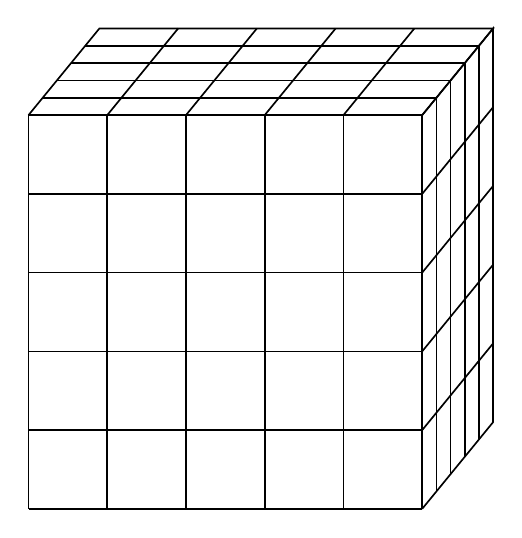
\begin{tikzpicture}[x=1cm,y=1cm,font=\normalsize,line width=.6pt]
\def\dx{0.9}
\def\dy{1.1}
% front 5x5 face
\draw (0,0) grid[xstep=1,ystep=1] (5,5);
% outer top and right faces
\draw (0,5) -- (\dx,5+\dy) -- (5+\dx,5+\dy) -- (5,5);
\draw (5,0) -- (5+\dx,\dy) -- (5+\dx,5+\dy) -- (5,5);
% top face subdivisions parallel to front edge
\foreach \k in {1,...,4} {
  \pgfmathsetmacro{\yy}{5+\k*\dy/5}
  \pgfmathsetmacro{\xxa}{\k*\dx/5}
  \pgfmathsetmacro{\xxb}{5+\k*\dx/5}
  \draw (\xxa,\yy) -- (\xxb,\yy);
}
% top face subdivisions parallel to depth
\foreach \i in {1,...,4} {
  \draw (\i,5) -- (\i+\dx,5+\dy);
}
% right face subdivisions: horizontal lines
\foreach \j in {1,...,4} {
  \draw (5,\j) -- (5+\dx,\j+\dy);
}
% right face subdivisions: depth-parallel verticals
\foreach \i in {1,...,4} {
  \pgfmathsetmacro{\xx}{5+\i*\dx/5}
  \pgfmathsetmacro{\yya}{\i*\dy/5}
  \pgfmathsetmacro{\yyb}{5+\i*\dy/5}
  \draw (\xx,\yya) -- (\xx,\yyb);
}
\end{tikzpicture}
